%! TEX root = ../main.tex
\chapter{研究设计}\label{chap:3}
\section{样本选择与数据来源}
\subsection{极端天气样本与数据}\label{sec:def}

气候代表了一个地区在一定时间跨度内所经历的天气状况的总体特征,揭示了一个地区的基本气象冷热、干湿特性,故而温度和降水是构成某一地区气候特征的两个最根本的气象要素\citep{alexander2006global}。在气候变化的大背景下,异常气候以及极端天气事件发生的可能性增加\citep{aigner2023summary,donat2017addendum},这其中极端强降水愈发频繁\citep{trenberth2010relationships}。在我国,极端天气事件如洪涝、干旱、台风、暴雪等自然灾害\citep{尹红2019基于},往往与极端强降水事件密切相关,给国家和人民带来了巨大的损失。因此,本文选取将极端降水作为极端天气事件的代表来,数据来源于国家气候中心,时间范围为1954年至2019年。

对于极端降雨强度的定义,国家标准 GB/T 33680-2017《暴雨灾害等级》中将日降水量超过 50mm 定义为暴雨,超过 250mm 定义为特大暴雨。然而,由于不同地区在气候特征和降水模式上存在显著差异,单一的数值标准可能无法全面反映极端降水事件的影响。参考国际气候变化检测和指数专家组(ETCCDI)采用分位数来定义极端天气的方法,将日降水量超过95th或99th百分位数的情况定义为极端降水\footnote{资料来源:UVIC,\url{https://etccdi.pacificclimate.org/list_27_indices.shtml}}。这种方法能够更好地适应不同地区的降水特征\citep{karl1999clivar},因此本文选择将极端降水天气定义为20年一遇的降水天气。

而关于极端降雨受灾范围的界定,结合降水数据和保单数据(见\ref{sec:data}),考虑到绝大多数保险标的与距离最近的气象站之间距离大多在50公里以内,平均距离不足30公里,如图\ref{fig:distance},因此本文将距离监测到极端降水的气象站20公里内的区域定义为灾区。而考虑到我国气象站分布间距基本在100公里以内,如图\ref{fig:locations},因此取气象站所覆盖的受灾半径最多为50公里,定义距离监测到极端降水的气象站20-50公里内的区域为近灾区,50公里以上的区域为远灾区。

\begin{figure}[H]
    \begin{minipage}{0.48\linewidth}
        \centering
        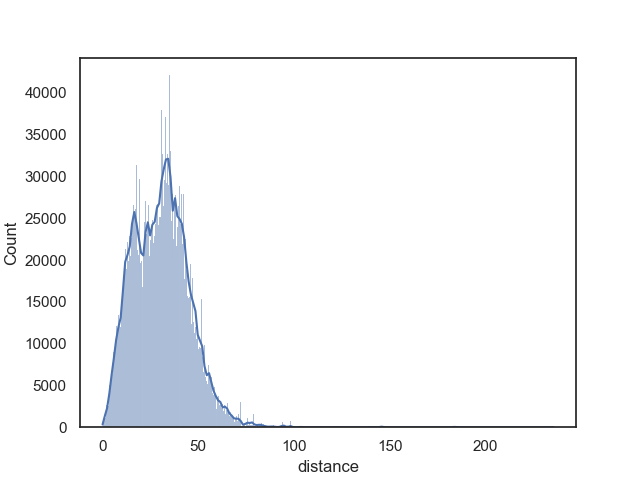
\includegraphics[width=\textwidth]{lib/img/distance.png}
        \caption{保险标与最临近气象站的距离分布(千米)}
        \label{fig:distance}
    \end{minipage}
    \begin{minipage}{0.48\linewidth}
        \centering
        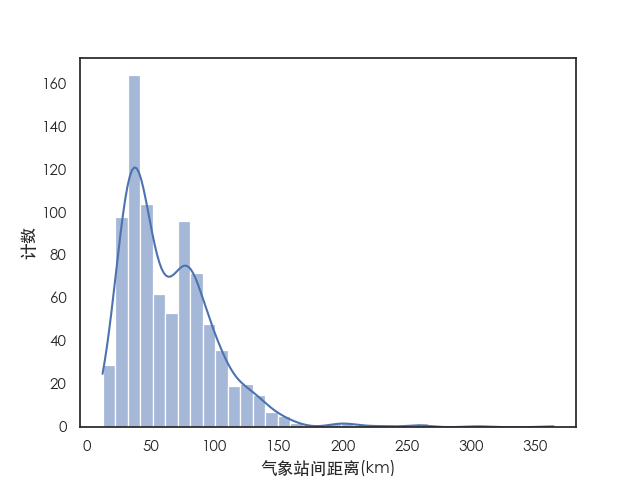
\includegraphics[width=\textwidth]{lib/img/locations_distance.png}
        \caption{气象站间距的地理位置分布(千米)}
        \label{fig:locations}
    \end{minipage}
\end{figure}

气象站地理位置分布如图\ref{fig:location}-图\ref{fig:end}所示。

\begin{figure}[H]
    \centering
    \begin{minipage}{0.48\linewidth}
        \includegraphics[width=\textwidth, trim=200 0 200 0]{lib/img/locations.png}
        \caption{所有气象站的地理位置分布}
        \label{fig:location}
    \end{minipage}
    \begin{minipage}{0.48\linewidth}
        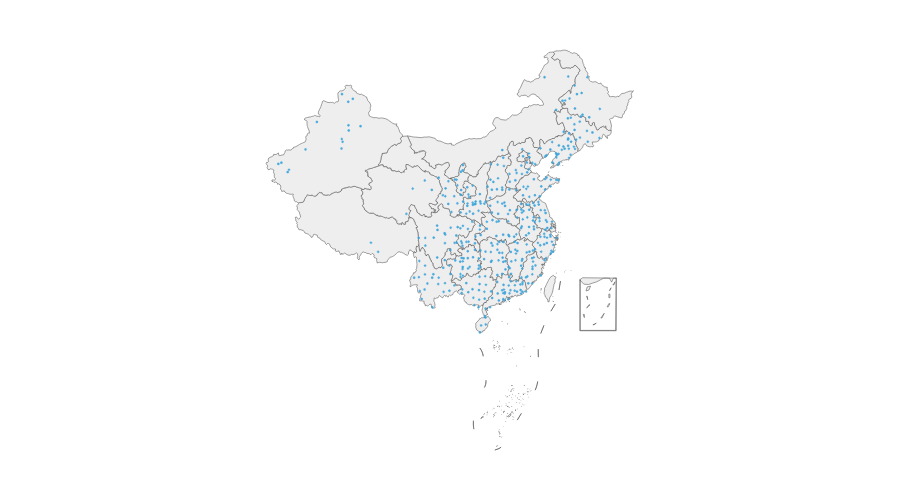
\includegraphics[width=\textwidth, trim=200 0 200 0]{lib/img/near.png}
        \caption{划分为灾区气象站的地理位置分布}
    \end{minipage}
\end{figure}
\begin{figure}[H]
    \begin{minipage}{0.48\linewidth}
        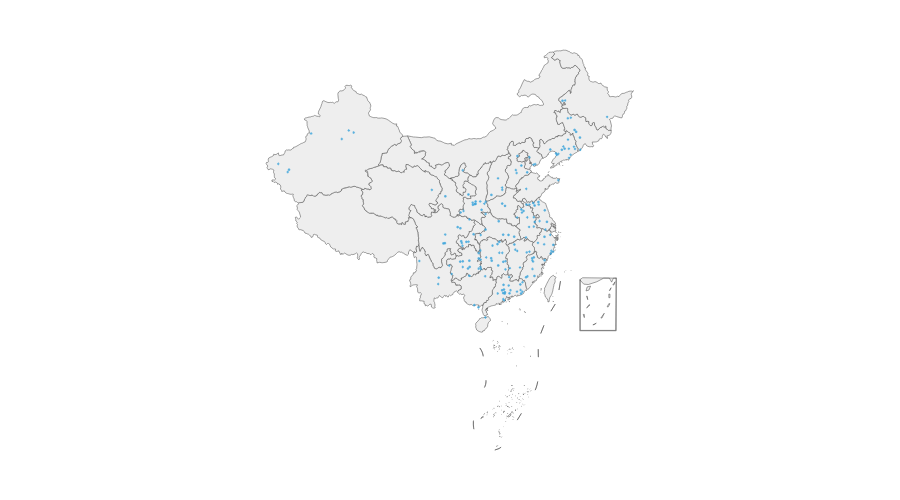
\includegraphics[width=\textwidth, trim=200 0 200 0]{lib/img/middle.png}
        \caption{划分为近灾区气象站的地理位置分布}
    \end{minipage}
    \begin{minipage}{0.48\linewidth}
        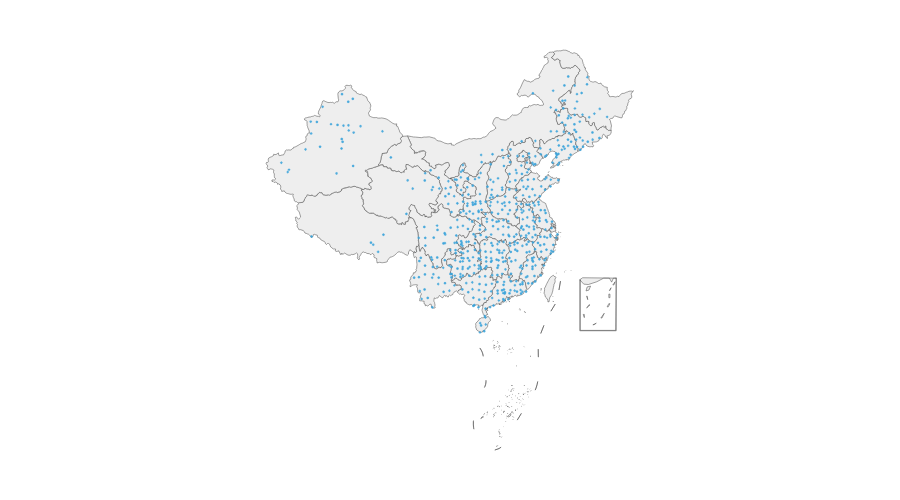
\includegraphics[width=\textwidth, trim=200 0 200 0]{lib/img/far.png}
        \caption{划分为非灾区气象站的地理位置分布}
        \label{fig:end}
    \end{minipage}
\end{figure}
\subsection{保险标的样本与数据}\label{sec:data}
本文以某财产保险公司1995年1月1日至2015年12月31日全国家财险承保理赔数据作为研究样本。

为了确保气象数据与标的样本之间的相关性,对样本基于距离进行了筛选,只选择了那些距离最近的气象站20公里以内的标的样本,然后再进行灾区、近灾区和非灾区划分进行分析。最终得到约了70万条可用于回归分析的数据。为降低异常值,影响本文对所有连续变量进行了1\%缩尾处理。

\section{模型设定与变量选取}
\subsection{变量定义}
为了更清晰地评估极端天气事件的影响,本文纳入一系列控制变量。这些变量包括:

\begin{enumerate}
    \item 是否历史投保:过去一年是否购买了家财险,可能影响他们对未来保险需求的决策。
    \item 保险财产购置价:反映了家庭财产的价值,通常财产价值越高,对风险的担心也越大,保险需求也越大。
    \item 建筑面积:建筑面积越大,需要更高的保险保额来覆盖潜在的风险。
    \item GDP增速:反应当地经济增长率,经济增长促进保险购买。
    \item 保险密度:反映了当地保险市场的发展程度,保险市场发展程度越高,家庭购买保险的可能性也越大。
    \item 保险深度:反映了家庭购买保险的程度,保单深度越高,家庭购买保险的可能性也越大。
\end{enumerate}

被解释变量与控制变量含义如表{tab:var}所示。
\begin{table}[H]
    \caption{变量定义表}\label{tab:var}
    \centering
    \begin{tabular}{@{}cccc@{}}
        \toprule
        变量类别                    & 变量名称         & 变量定义    & 变量解释                \\ \midrule
        被解释变量                   & Coverage     & 保额      & 保险金额                \\ \midrule
        \multirow{3}{*}{主要解释变量} & Disaster     & 灾区      & 是否处于极端降水监测点20公里内    \\ \cmidrule(l){2-4}
                                & Neighbor     & 近灾区     & 是否处于极端降水监测点20-50公里内 \\ \cmidrule(l){2-4}
                                & Post         & 降水发生时间  & 是否在极端降水发生后投保        \\
        \midrule
        \multirow{3}{*}{控制变量}   & Prem\_before & 历史投保    & 保险标的是否有投保记录         \\ \cmidrule(l){2-4}
                                & Price        & 保险财产购置价 & 保险标的资产购置价           \\ \cmidrule(l){2-4}
                                & Area         & 建筑面积    & 保险标的建筑面积            \\ %\cmidrule(l){2-4}
        % & Claim       & 是否理赔    & 该保单是否发生理赔            \\
        \bottomrule
    \end{tabular}
\end{table}


\subsection{模型设定}
极端天气事件是一个外生冲击,在时空上的分布是随机的,因此本文采用了DID回归来估计极端天气事件对家庭财产保险的影响。本文设定实验组和对照组,实验组为受灾区或近灾区,对照组为未受灾区。

针对假设\ref{hyp:2},建立如下双重差分模型:

\begin{equation}
    \log\text{Coverage}=\alpha+\beta_1\text{Disaster}+\beta_2\text{Post}+\beta_3\text{Disaster}\times\text{Post}+\beta\text{Controls}+\varepsilon
    \label{eq:DID_1}
\end{equation}

针对假设\ref{hyp:3},建立如下双重差分模型:

\begin{equation}
    \log\text{Coverage}=\alpha+\beta_1\text{Neighbor}+\beta_2\text{Post}+\beta_3\text{Neighbor}\times\text{Post}+\beta\text{Controls}+\varepsilon
    \label{eq:DID_2}
\end{equation}

TODO:这两个模型后面需要增加一段,对上面模型进行说明,具体请参考塔佳宜论文中的相应部分。他那里面七是季度,所以比较多,你这里面一期就是一年。另外你公式中没有下标,具体你也参考他的论文中的模型
